\section{Caso prático}\label{sec:caso}

\begin{frame}{Comparativos}
Duas tarefas, dois conjuntos \alert{disponíveis no scikit-learn} (sem download):
\begin{itemize}
  \item \textbf{Classificação}: Iris ($150$ flores, $4$ medidas, $3$ espécies).
  \item \textbf{Regressão}: \emph{diabetes} ($442$ pacientes, $10$ variáveis, resposta: progressão da doença).
\end{itemize}
Pergunta: \alert{quando vale a pena usar árvores}, comparadas com \alert{baselines} (regressão linear/logística, KNN, LDA, SVM)?
\begin{enumerate}
  \item Protocolo de avaliação.
  \item Classificação: árvores $\times$ baselines.
  \item Regressão: árvores (e ensembles) $\times$ baselines.
  \item Duas propriedades das árvores: \alert{escala} e \alert{rotação} dos eixos.
  \item Resumo: o que levar para a prática.
\end{enumerate}
\end{frame}

\begin{frame}{Protocolo de avaliação}
\begin{itemize}
  \item \alert{Repetir} a divisão treino/teste ($75/25$): $100$ vezes no Iris (estratificado), $50$ no \emph{diabetes}. Com $38$ flores de teste, uma observação vale $2{,}6$ p.p.; uma única divisão não decide.
  \item Relatamos \alert{média $\pm$ desvio-padrão} entre as divisões. Diferenças menores que o desvio-padrão \alert{não} devem ser lidas como superioridade.
  \item Pré-processamento \alert{dentro} do \texttt{Pipeline}: a padronização (para KNN, SVM e regressão logística) é ajustada só com o treino de cada divisão, evitando \emph{vazamento}.
  \item Hiperparâmetros \alert{fixados antes}, sem ajuste fino para nenhum método (ver código). Um ajuste por validação cruzada pode mudar a ordem entre métodos próximos.
\end{itemize}
\end{frame}

\begin{frame}[fragile]{Classificação (Iris): árvores $\times$ baselines}
\centering\small
\begin{tabular}{@{}lcc@{}}
\toprule
Método & Acurácia & F1 macro \\
\midrule
Regressão logística & 0,954 $\pm$ 0,028 & 0,954 $\pm$ 0,028 \\
KNN ($k=5$) & 0,950 $\pm$ 0,031 & 0,950 $\pm$ 0,030 \\
LDA & 0,982 $\pm$ 0,018 & 0,982 $\pm$ 0,018 \\
SVM (RBF) & 0,960 $\pm$ 0,028 & 0,960 $\pm$ 0,028 \\
Árvore (prof.\ 3) & 0,943 $\pm$ 0,032 & 0,943 $\pm$ 0,032 \\
Árvore (completa) & 0,946 $\pm$ 0,033 & 0,946 $\pm$ 0,033 \\
\bottomrule
\end{tabular}


\vspace{4pt}
\raggedright
\begin{itemize}
  \item \alert{LDA lidera} ($0{,}982$): as classes são quase \alert{linearmente separáveis} e aproximadamente gaussianas com covariâncias parecidas, o que o LDA supõe.
  \item SVM, regressão logística e KNN: $0{,}950$--$0{,}960$. As árvores: $0{,}943$--$0{,}946$, \alert{abaixo} dos baselines, mas por menos de $2$ desvios-padrão ($\approx0{,}03$).
  \item A árvore de profundidade $3$ empata com a completa e cabe em um slide: aqui a árvore compra \alert{interpretabilidade} quase sem custo.
\end{itemize}
{\scriptsize Código: \texttt{01\_baselines\_classificacao.py}.}
\end{frame}

\begin{frame}{Regressão (\emph{diabetes}): árvores $\times$ baselines}
\centering\small
\begin{tabular}{@{}lcc@{}}
\toprule
Método & RMSE & $R^2$ \\
\midrule
Regressão linear & 54,9 $\pm$ 2,7 & 0,47 $\pm$ 0,05 \\
KNN ($k=15$) & 57,0 $\pm$ 3,2 & 0,43 $\pm$ 0,05 \\
SVR (RBF, $C=100$) & 57,9 $\pm$ 3,9 & 0,41 $\pm$ 0,08 \\
Árvore (prof.\ 3) & 63,0 $\pm$ 3,7 & 0,30 $\pm$ 0,10 \\
Árvore (completa) & 80,1 $\pm$ 4,8 & -0,12 $\pm$ 0,15 \\
Floresta ($B=300$) & 57,3 $\pm$ 3,6 & 0,43 $\pm$ 0,08 \\
Gradient boosting & 56,7 $\pm$ 3,1 & 0,44 $\pm$ 0,06 \\
\bottomrule
\end{tabular}


\vspace{4pt}
\raggedright
\begin{itemize}
  \item A \alert{regressão linear} vence ($54{,}9$): a relação resposta--variáveis é aproximadamente linear.
  \item \alert{Árvore completa}: RMSE $80{,}1$ e $R^2<0$, \alert{pior que prever a média}. Poda (prof.\ $3$) melhora para $63{,}0$.
  \item Floresta e gradient boosting ($56{,}7$--$57{,}3$) recuperam quase todo o terreno perdido pela árvore, e ficam a $\approx2$ pontos da regressão linear, dentro de $1$ desvio-padrão.
\end{itemize}
{\scriptsize Código: \texttt{02\_baselines\_regressao.py}. Hiperparâmetros fixados antes, sem ajuste.}
\end{frame}

\begin{frame}{Propriedade 1: indiferença à escala das variáveis}
\begin{columns}[T]
\column{0.5\textwidth}
\centering\footnotesize
\begin{tabular}{@{}lcc@{}}
\toprule
Método & Original & Variável 1 $\times\,1000$ \\
\midrule
KNN & 0,964 & 0,759 \\
SVM (RBF) & 0,959 & 0,684 \\
Regressão logística & 0,963 & 0,959 \\
LDA & 0,981 & 0,981 \\
Árvore (prof.\ 3) & 0,939 & 0,939 \\
\bottomrule
\end{tabular}


\vspace{4pt}
{\scriptsize Acurácia média no Iris ($50$ divisões), \alert{sem} padronizar; a variável $1$ (comprimento da sépala) é multiplicada por $1000$.}
\column{0.47\textwidth}
\small
\begin{itemize}
  \item \alert{KNN} e \alert{SVM} dependem de \alert{distâncias}: a variável $\times1000$ domina e a acurácia cai $20$--$28$ p.p.
  \item A \alert{árvore} só usa a \alert{ordem} dos valores em cada variável: a partição dos dados de treino \alert{não muda}.
  \item LDA é invariante a escalas lineares. A regressão logística mal muda ($0{,}963\to0{,}959$): a regularização $L_2$ depende da escala.
\end{itemize}
\end{columns}
\vspace{4pt}
\begin{block}{Consequência}
Árvores dispensam padronização, e qualquer transformação \alert{estritamente crescente} de uma variável (log, raiz) deixa a partição do treino igual.
\end{block}
\end{frame}

\begin{frame}{Propriedade 2: a rotação dos eixos}
\centering
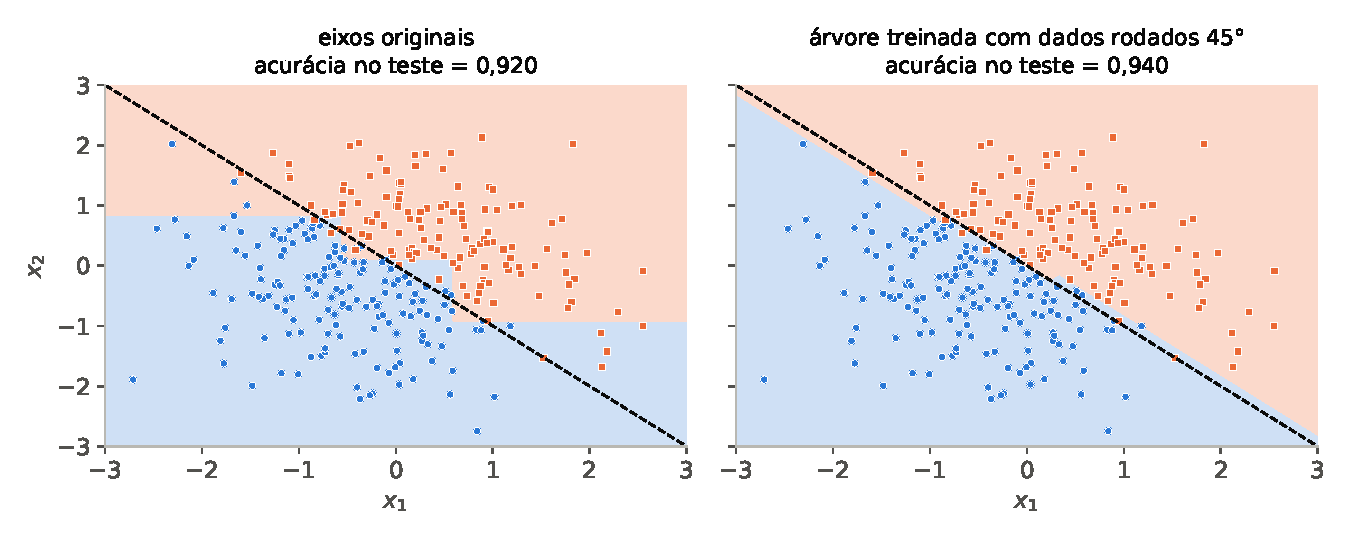
\includegraphics[width=0.62\linewidth]{../python/comparativo/figures/rotacao.pdf}
\vspace{2pt}
\begin{itemize}
  \item Cortes $x_j\le\tau$ dão fronteiras \alert{paralelas aos eixos}: uma fronteira \alert{diagonal} ($x_1+x_2=0$) vira uma \alert{escada}.
  \item Sintéticos ($50$ divisões, prof.\ $3$): árvore $0{,}891$; com dados \alert{rodados $45^\circ$} $0{,}968$; regressão logística $0{,}976$.
  \item Mas depende da \alert{geometria}: no Iris, rodar os $4$ eixos por uma matriz ortogonal aleatória \alert{não} prejudicou ($0{,}939\to0{,}937$).
\end{itemize}
{\scriptsize Código: \texttt{04\_rotacao.py}, \texttt{fig\_rotacao.py}.}
\end{frame}

\begin{frame}{Resumo: o que levar para a prática}
\small
\centering
\begin{tabular}{@{}p{0.2\textwidth}p{0.24\textwidth}p{0.24\textwidth}p{0.2\textwidth}@{}}
\toprule
 & \textbf{Árvore} & \textbf{Linear / LDA} & \textbf{KNN / SVM}\\
\midrule
Escala das variáveis & indiferente & LDA: indiferente & \alert{sensível}\\
Rotação dos eixos & \alert{sensível} (fronteira diagonal) & indiferente & indiferente\\
Interpretação & alta (regras) & alta (coeficientes) & baixa\\
Extrapolação & constante (degraus) & linear & tende a constante\\
\bottomrule
\end{tabular}

\vspace{6pt}
\raggedright
\begin{itemize}
  \item Nos dois conjuntos, \alert{uma árvore sozinha não vence} os baselines; floresta e boosting chegam perto.
  \item Árvores costumam brilhar com variáveis em unidades distintas, interações e mistura de tipos (que o Iris e o \emph{diabetes} não testam); sempre \alert{compare com um baseline simples}.
\end{itemize}
\end{frame}
